\documentclass{article}

% if you need to pass options to natbib, use, e.g.:
%     \PassOptionsToPackage{numbers, compress}{natbib}
% before loading neurips_2019

% ready for submission
% \usepackage{neurips_2019}

% to compile a preprint version, e.g., for submission to arXiv, add add the
% [preprint] option:
     \usepackage[preprint]{neurips_2019}

% to compile a camera-ready version, add the [final] option, e.g.:
%     \usepackage[final]{neurips_2019}

% to avoid loading the natbib package, add option nonatbib:
%     \usepackage[nonatbib]{neurips_2019}

\usepackage[utf8]{inputenc} % allow utf-8 input
\usepackage[T1]{fontenc}    % use 8-bit T1 fonts
\usepackage{hyperref}       % hyperlinks
\usepackage{url}            % simple URL typesetting
\usepackage{booktabs}       % professional-quality tables
\usepackage{amsfonts}       % blackboard math symbols
\usepackage{nicefrac}       % compact symbols for 1/2, etc.
\usepackage{microtype}      % microtypography

% Not part of the offical NeurIPS template
\usepackage{censor}
\usepackage{amssymb}
\usepackage{amsthm}
\usepackage{mathtools}
\usepackage{caption}
\usepackage{subcaption}
\usepackage{caption}
\usepackage{csquotes}
\usepackage{layouts}
\usepackage{float}
\usepackage{todonotes}
\usepackage{enumitem}

% Algorithms
\usepackage{algorithm}
\usepackage[noend]{algpseudocode}
\algnewcommand{\Let}[2]{\State #1 $\gets$ #2}
\algrenewcommand\Call[2]{\textproc{#1}(#2)}

% Kabel Tables
\usepackage{multirow}
\usepackage{tabu}

\title{Neural Arithmetic Units}

% The \author macro works with any number of authors. There are two commands
% used to separate the names and addresses of multiple authors: \And and \AND.
%
% Using \And between authors leaves it to LaTeX to determine where to break the
% lines. Using \AND forces a line break at that point. So, if LaTeX puts 3 of 4
% authors names on the first line, and the last on the second line, try using
% \AND instead of \And before the third author name.

\author{%
  Andreas Madsen$^{\dag\ddag}$ \\
  \texttt{amwebdk@gmail.com}
  \AND
  Alexander Rosenberg Johansen$^{\dag}$ \\
  \texttt{aler@dtu.dk} \\
  \AND
  Who else? \\
  \\
$^\dag$Technical University of Denmark \quad
$^\ddag$Computationally Demanding
}

\begin{document}
\StopCensoring % NOTE, remove for peer-review to ensure anonymity.

\maketitle

\begin{abstract}
%What’s the domain?
Arithmetic problems are solved by rules and axioms, which presents a unique challenge for machine learning models.
%What’s the issue?
Neural networks have, with millions and sometimes billions of parameters, an ability to approximate complex functions.
However, when extrapolating on out-of-distribution samples neural networks often fail to learn the underlying logic.
%What’s your contribution?
We propose a plug-and-play differentiable neural unit that can be trained using stochastic gradient descent to learn addition, subtraction and multiplication.
Our proposed Neural Addition Unit (NAU) and Neural Multiplication Unit (NMU) rely on weight constraints to learn rules and extrapolate well beyond the training distribution.
%Why is it novel?
%What’s interesting about it?
The proposed NAU and NMU are inspired by the Neural Arithmetic Logic Unit (NALU).
We find that replacing the nonlinearities in the weight matrix with a clipped linear function and fundamentally reformulate the multiplication unit is crucial for converging consistently.
%How does it perform?
Through analytic and empirical analysis we justify how the NAU and NMU improve the Neural Arithmetic Logic Unit (NALU) and standard multi-layer perceptron (MLP) models.
Our models have fewer parameters, convergence more consistently, learns faster and have more meaningful discrete values than the NALU.\footnote{In the interest of scientific integrity, we have made the code for all experiments, and more, available on GitHub: \censor{\url{https://github.com/AndreasMadsen/stable-nalu}}.}
\end{abstract}

\section{Introduction}
When studying intelligence, insects, reptiles, and humans have been found to possess neurons with the capacity to hold integers, real numbers, and perform arithmetic operations \cite{nieder-neuronal-number,rugani-arithmetic-chicks,gallistel-numbers-in-brain}.
In our quest to mimic intelligence, we have put much faith in neural networks, which in turn has provided unparalleled and often superhuman performance in tasks requiring high cognitive abilities \cite{natureGo,bert,openai-learning-dexterous}.
However, when using neural networks to solve simple arithmetic problems, such as counting, multiplication, or comparison, they systematically fail to extrapolate onto unseen ranges \cite{stillNotSystematic,suzgun2019evaluating,trask-nalu}.
The absence of inductive bias makes it difficult for neural networks to extrapolate well on arithmetic tasks as they lack the underlying logic to represent the required operations.

A neural component that can solve arithmetic problems should be able to: take an arbitrary hidden input, learn to select the appropriate elements, and apply the desired arithmetic operation.
A recent attempt to achieve this goal is the Neural Arithmetic Logic Unit (NALU) by \citet{trask-nalu}.

The NALU models the inductive bias explicitly via two sub-units: the $\text{NAC}_{+}$ for addition/subtraction and the $\text{NAC}_{\bullet}$ for multiplication/division.
The sub-units are softly gated between, using a sigmoid function, to exclusively select one of the sub-units.
However, we find that the soft gating-mechanism and the $\text{NAC}_{\bullet}$ are fragile and hard to learn.

In this paper, we analyze and improve upon the $\text{NAC}_{+}$ and $\text{NAC}_{\bullet}$ with respect to addition, subtraction, and multiplication.
Our proposed improvements, namely the Neural Addition Unit (NAU) and Neural Multiplication Unit (NMU), are more theoretically founded and improve performance regarding stability, speed of convergence, and interpretability of weights.
Most importantly, the NMU supports both negative and small numbers and a large hidden input-size, which is paramount as neural networks are overparameterized and hidden values are often unbounded.

The improvements, which are based on a theoretical analysis of the NALU and its components, are achieved by a simplification of the parameter matrix for a better gradient signal, a sparsity regularizer, and a new multiplication unit that can be optimally initialized.
The NMU does not support division.
However, we find that the $\text{NAC}_{\bullet}$ in practice also only supports multiplication and cannot learn division (theoretical analysis on division discussed in section \ref{sssec:nac-mul}).

To analyze the impact of each improvement, we introduce several variants of the $\text{NAC}_{\bullet}$.
We find that allowing division makes optimization for multiplication harder, linear and regularized weights improve convergence, and the NMU way of multiplying is critical when increasing the hidden size.

Furthermore, we improve upon existing benchmarks in \citet{trask-nalu} by expanding the ``simple function task'', expanding ``MNIST Counting and Arithmetic Tasks'' with a multiplicative task, and using an improved success-criterion \citet{maep-madsen-johansen-2019}.
This success-criterion is important because the arithmetic layers are solving a logical problem.
We propose the MNIST multiplication variant as we want to test the NMU’s and $\text{NAC}_{\bullet}$’s ability to learn from real data and extrapolate.

\begin{figure}[t]
\centering
\vspace{-1em}
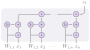
\includegraphics[scale=0.65]{graphics/nmu.pdf}
\caption{Visualization of NMU for a single output scalar $z_1$, this construction repeats for every element in the output vector $\mathbf{z}$.}
\end{figure}

\subsection{Learning a 10 parameter function}
Consider the static function $t = (x_1 + x_2) \cdot (x_1 + x_2 + x_3 + x_4)$ for $x \in \mathbb{R}^4$. To illustrate the ability of $\mathrm{NAC}_{\bullet}$, NALU, and our proposed NMU, we conduct 100 experiments for each model, where we attempt to fit this function. Table \ref{tab:very-simple-function-results} shows that NMU has a higher success rate and converge faster.
\begin{table}[!h]

\caption{\label{tab:very-simple-function-results}Comparison of the success-rate, when the model converged, and the sparsity error for all weight matrices, with 95\% confidence interval on the $t = (x_1 + x_2) \cdot (x_1 + x_2 + x_3 + x_4)$ task. Each value is a summary of 100 different seeds.}
\centering
\begin{tabular}{crllll}
\toprule
\multicolumn{1}{c}{Op} & \multicolumn{1}{c}{Model} & \multicolumn{1}{c}{Success} & \multicolumn{2}{c}{Solved at} & \multicolumn{1}{c}{Sparsity error} \\
\cmidrule(l{3pt}r{3pt}){1-1} \cmidrule(l{3pt}r{3pt}){2-2} \cmidrule(l{3pt}r{3pt}){3-3} \cmidrule(l{3pt}r{3pt}){4-5} \cmidrule(l{3pt}r{3pt}){6-6}
 &  & Rate & Median & Mean & Mean\\
\midrule
 & $\mathrm{NAC}_{\bullet}$ & $13\% {~}^{+8\%}_{-5\%}$ & $5.5 \cdot 10^{4}$ & $5.9 \cdot 10^{4} {~}^{+7.8 \cdot 10^{3}}_{-6.6 \cdot 10^{3}}$ & $7.5 \cdot 10^{-6} {~}^{+2.0 \cdot 10^{-6}}_{-2.0 \cdot 10^{-6}}$\\

\nopagebreak
 & NALU & $26\% {~}^{+9\%}_{-8\%}$ & $7.0 \cdot 10^{4}$ & $7.8 \cdot 10^{4} {~}^{+6.2 \cdot 10^{3}}_{-8.6 \cdot 10^{3}}$ & $9.2 \cdot 10^{-6} {~}^{+1.7 \cdot 10^{-6}}_{-1.7 \cdot 10^{-6}}$\\

\nopagebreak
\multirow{-3}{*}{\centering\arraybackslash $\bm{\times}$} & NMU & $\mathbf{94\%} {~}^{+3\%}_{-6\%}$ & $\mathbf{1.4 \cdot 10^{4}}$ & $\mathbf{1.4 \cdot 10^{4}} {~}^{+2.2 \cdot 10^{2}}_{-2.1 \cdot 10^{2}}$ & $\mathbf{2.6 \cdot 10^{-8}} {~}^{+6.4 \cdot 10^{-9}}_{-6.4 \cdot 10^{-9}}$\\
\bottomrule
\end{tabular}
\end{table}


\section{Improving NAC and NALU}

The NALU from \cite{trask-nalu} is a neural unit capable of doing either exact addition or multiplication, controlled by a sigmoid-gating-mechanism. The addition part is trivial, as this is just a matrix multiplication $\mathbf{a} = \mathbf{W}\mathbf{x}$. The only special part is that the weight matrix $\mathbf{W}$ is constrained to be between $-1$ and $1$. This this done using a $\mathbf{W} = \mathrm{tahn}({\hat{\mathbf{W}}}) \sigma({\hat{\mathbf{M}}})$ construction. Meaning that the weight matrix $\mathbf{W}$ is not trained directly, but computed from two auxiliary weight matrices. The core idea is that $\hat{\mathbf{W}}$ controls the sign and $\hat{\mathbf{M}}$ controls if the weight is zero. One of their core claims, is that this weight matrix construction have a sparse bias, which improves extrapolation for cases where a sparse weight is part of the underlying model.

For the multiplication, an exponential-log transformation is used in order to do exact multiplication (within $\epsilon$ precision) using a matrix multiplication, $\mathbf{m} = \exp(\mathbf{W} \log(|\mathbf{x}| + \epsilon))$.

The addition unit (originally named NAC), and the multiplication unit are in themselves theoretically applicable in any neural network as well as being differentiable. The NALU, then combines them using a sigmoid-gating-mechanism\footnote{The lack of bias term is not a typo. Our preliminary investigations suggests that this is a hack to increase extrapolation of the gate. However in this paper the focus is only arithmetic operators themself.} $\mathbf{g} = \sigma(\mathbf{G} \mathbf{x})$ that chooses softly between addition and multiplication $\mathbf{z} = \mathbf{g} \odot \mathbf{a} + (1 - \mathbf{g}) \odot \mathbf{m}$.

In terms of the theory, the Original NALU paper \cite{trask-nalu} does not discuss anything more than mentioned so-far in this paper. To aid discussion of why this particular construction problematic, and also suggests improvements which will be empirically validated later, the NAC and its multiplication variant is re-formulated using scalar notation.

\begin{equation}
\begin{aligned}
&W_{h_\ell, h_{\ell-1}} = \tanh(\hat{W}_{h_\ell, h_{\ell-1}}) \sigma(\hat{M}_{h_\ell, h_{\ell-1}}) \\
\textrm{NAC}_+:\ &z_{h_\ell} = \sum_{h_{\ell-1}=1}^{H_{\ell-1}} W_{h_{\ell}, h_{\ell-1}} z_{h_{\ell-1}} \\
\textrm{NAC}_\bullet:\ &z_{h_\ell} = \exp\left(\sum_{h_{\ell-1}=1}^{H_{\ell-1}} W_{h_{\ell}, h_{\ell-1}} \log(|z_{h_{\ell-1}}| + \epsilon) \right)
\end{aligned}
\end{equation}

\subsection{Weight matrix construction}

The weight matrix constructions $\mathrm{tahn}({\hat{\mathbf{W}}}) \sigma({\hat{\mathbf{M}}})$ have a few issues worth mentioning. First, the loss gradient with respect to the weight matrices, can without loss of generality, easily be derived to:

\begin{equation}
\begin{aligned}
\frac{\partial \mathcal{L}}{\partial \hat{W}_{h_{\ell-1},h_\ell}} &= \frac{\partial \mathcal{L}}{\partial W_{h_{\ell-1},h_\ell}} (1 - \tanh^2(\hat{W}_{h_{\ell-1},h_\ell})) \sigma(\hat{M}_{h_{\ell-1},h_\ell}) \\
\frac{\partial \mathcal{L}}{\partial \hat{M}_{h_{\ell-1},h_\ell}} &= \frac{\partial \mathcal{L}}{\partial W_{h_{\ell-1},h_\ell}} \tanh(\hat{W}_{h_{\ell-1},h_\ell}) \sigma(\hat{M}_{h_{\ell-1},h_\ell}) (1 - \sigma(\hat{M}_{h_{\ell-1},h_\ell}))
\end{aligned}
\end{equation}

This reveals that this construction is particularly problematic, as $E[\mathrm{tahn}(\hat{W}_{h_{\ell-1},h_\ell})] = 0$ when $E[\hat{W}_{h_{\ell-1},h_\ell}] = 0$. Initializing $\hat{W}_{h_{\ell-1},h_\ell}$ to have zero expectation, is not just common choice but necessary in order to achieve $E[W_{h_{\ell-1},h_\ell}] = 0$, which is necessary to get desired property $E[z_{h_\ell}] = 0$ in linear units such as as the NAC \cite{glorot-initialization}.

The NALU \cite{trask-nalu} paper also claims that this weight matrix construction, creates a bias for ${-1, 0, 1}$. However, they provide no empirically or theoretical evidence to support that. In our own empirical investigation as seen in the experiments section, we also find no support for that claim.

To improve on both of these failings, we propose a simple clamped linear construction instead, that is regularize to have the desired bias of $\{-1, 0, 1\}$ and have gradient outside of $[-1, 1]$.

\begin{equation}
\begin{aligned}
&W_{h_{\ell-1},h_\ell} = \min(\max(\hat{W}_{h_{\ell-1},h_\ell}, -1), 1), \\
&\mathcal{R}_{\ell,\mathrm{bias}} = \frac{1}{H_\ell + H_{\ell-1}} \sum_{h_\ell=1}^{H_\ell} \sum_{h_{\ell-1}=1}^{H_{\ell-1}} \hat{W}_{h_{\ell-1},h_\ell}^2 (1 - |\hat{W}_{h_{\ell-1},h_\ell}|)^2 \\
&\mathcal{R}_{\ell,\mathrm{oob}} = \frac{1}{H_\ell + H_{\ell-1}} \sum_{h_\ell=1}^{H_\ell} \sum_{h_{\ell-1}=1}^{H_{\ell-1}} \max(|\hat{W}_{h_{\ell-1},h_\ell}| - 1, 0)^2 \\
\textrm{NAU}:\ &z_{h_\ell} = \sum_{h_{\ell-1}=1}^{H_{\ell-1}} W_{h_{\ell}, h_{\ell-1}} z_{h_{\ell-1}} \\\end{aligned}
\end{equation}

Note that while the bias regularizer $\mathcal{R}_{\ell,\mathrm{bias}}$ also regularize $\hat{W}_{h_{\ell-1},h_\ell}$ to not be outside of $[-1, 1]$, one may choose a small regularization constant for this, or scale it up gradually as done in the experiments later. However, $\mathcal{R}_{\ell,\mathrm{oob}}$ should always be present as it is never desired to have $\hat{W}_{h_{\ell-1},h_\ell} \not\in [-1, 1]$.

\subsection{Multiplication unit}

The multiplication unit has its own issues. It should be easy to see that when $|z_{h_{\ell-1}}|$ is near zero and when $\hat{W}_{h_{\ell-1},h_\ell}$ is near $-1$ the $z_{h_\ell}$ value explodes. However, the issue extends beyond a weight near $-1$ as is revealed in the gradients, especially the backpropergation term $\frac{\partial z_{h_\ell}}{\partial z_{h_{\ell-1}}}$:

\begin{equation}
\begin{aligned}
\frac{\partial \mathcal{L}}{\partial W_{h_{\ell}, h_{\ell - 1}}} &= \frac{\partial \mathcal{L}}{\partial z_{h_\ell}} \frac{\partial z_{h_\ell}}{\partial W_{h_{\ell}, h_{\ell - 1}}} = \frac{\partial \mathcal{L}}{\partial z_{h_\ell}} z_{h_\ell} \log(|z_{h_{\ell-1}}| + \epsilon) \\
\frac{\partial \mathcal{L}}{\partial z_{h_{\ell-1}}} &= \sum_{h_\ell = 1}^{H_\ell} \frac{\partial \mathcal{L}}{\partial z_{h_\ell}} \frac{\partial z_{h_\ell}}{\partial z_{h_{\ell-1}}} = \sum_{h_\ell = 1}^{H_\ell} \frac{\partial \mathcal{L}}{\partial z_{h_\ell}} z_{h_\ell} W_{h_\ell, h_{\ell-1}} \frac{\mathrm{sign}(z_{h_{\ell-1}})}{|z_{h_{\ell-1}}| + \epsilon}
\end{aligned}
\end{equation}

In should be clear from $\frac{\mathrm{sign}(z_{h_{\ell-1}})}{|z_{h_{\ell-1}}| + \epsilon}$ that for $z_{h_{\ell-1}}$ near zero, the backpropagation term will not only explode, but can oscillate between a large postive value and large negative value, which is very problematic in optimization \cite{adam-optimization}. This issue does not only exists for $|z_{h_{\ell-1}}| < \epsilon$, which may have a small probability if $z_{h_{\ell-1}}$ has a wide distribution. But is can also be an issue for values outside of this interval as seen in figure \ref{fig:nac-mul-eps-issue}.

\begin{figure}[H]
\centering
\begin{subfigure}{.33\textwidth}
  \centering
  \includegraphics[width=\linewidth]{graphics/nac-mul-eps-1em7.png}
  \caption{$\epsilon = 10^{-7}$}
\end{subfigure}%
\begin{subfigure}{.33\textwidth}
  \centering
  \includegraphics[width=\linewidth]{graphics/nac-mul-eps-1em1.png}
  \caption{$\epsilon = 0.1$}
\end{subfigure}
\begin{subfigure}{.33\textwidth}
  \centering
  \includegraphics[width=\linewidth]{graphics/nac-mul-eps-1.png}
  \caption{$\epsilon = 1$}
\end{subfigure}
\caption{RMS loss curvature for a $\mathrm{NAC}_{+}$ layer followed by a $\mathrm{NAC}_{\bullet}$ layer. The weight matrices constrained are to $\mathbf{W}_1 = \left[\protect\begin{smallmatrix}
w_1 & w_1 & 0 & 0 \\
w_1 & w_1 & w_1 & 0
\protect\end{smallmatrix}\right]$, $\mathbf{W}_2 = \left[\protect\begin{smallmatrix}
w_2 & w_2
\protect\end{smallmatrix}\right]$. The problem is $x = \left(1, 1.5, 2, 2\right), t = 11.25$. Desired solution is $w_1 = w_2 = 1$, although this problem have additional undesired solutions.}
\label{fig:nac-mul-eps-issue}
\end{figure}

These observations are particular problematic when considering that $E[z_{h_{\ell-1}}] = 0$ is a desired property when initializing \cite{glorot-initialization}. An alternative multiplication operator must thus be able to not explode for $z_{h_{\ell-1}}$ near zero. To that end we propose a new neural multplication units (NMU): 

\begin{equation}
\begin{aligned}
&W_{h_{\ell-1},h_\ell} = \min(\max(\hat{W}_{h_{\ell-1},h_\ell}, 0), 1), \\
&\mathcal{R}_{\ell,\mathrm{bias}} = \frac{1}{H_\ell + H_{\ell-1}} \sum_{h_\ell=1}^{H_\ell} \sum_{h_{\ell-1}=1}^{H_{\ell-1}} \hat{W}_{h_{\ell-1},h_\ell}^2 (1 - \hat{W}_{h_{\ell-1},h_\ell})^2 \\
&\mathcal{R}_{\ell,\mathrm{oob}} = \frac{1}{H_\ell + H_{\ell-1}} \sum_{h_\ell=1}^{H_\ell} \sum_{h_{\ell-1}=1}^{H_{\ell-1}} \max\left(\left|\hat{W}_{h_{\ell-1},h_\ell} - \frac{1}{2}\right| - \frac{1}{2}, 0\right)^2 \\
\textrm{NMU}:\ &z_{h_\ell} = \prod_{h_{\ell-1}=1}^{H_{\ell-1}} \left(W_{h_{\ell-1},h_\ell} z_{h_{\ell-1}} + 1 - W_{h_{\ell-1},h_\ell} \right)
\end{aligned}
\end{equation}

This units does not support division. But supporting division is likely infeasible if $z_{h_{\ell-1}}$ near zero should not cause explosions. The NALU paper also shows that division doesn't work well for their unit, hence very little is lost here \cite{trask-nalu}. On the other hand, this unit construction understand the difference between a negative and a positive $z_{h_{\ell-1}}$ values, which should be considered an added bonus,as this allows extrapolations into the negative input range.

The gradients weight gradient and backpropagation term of the NMU are:
\begin{equation}
\begin{aligned}
\frac{\partial \mathcal{L}}{\partial W_{h_{\ell}, h_{\ell - 1}}} &= \frac{\partial \mathcal{L}}{\partial z_{h_\ell}} \frac{\partial z_{h_\ell}}{\partial W_{h_{\ell}, h_{\ell - 1}}} = \frac{\partial \mathcal{L}}{\partial z_{h_\ell}} \frac{z_{h_\ell}}{W_{h_{\ell-1},h_\ell} z_{h_{\ell-1}} + 1 - W_{h_{\ell-1},h_\ell}} \left(z_{h_{\ell-1}} - 1\right) \\
\frac{\partial \mathcal{L}}{\partial z_{h_{\ell-1}}} &= \sum_{h_\ell = 1}^{H_\ell} \frac{\partial \mathcal{L}}{\partial z_{h_\ell}} \frac{\partial z_{h_\ell}}{\partial z_{h_{\ell-1}}} = \sum_{h_\ell = 1}^{H_\ell} \frac{z_{h_\ell}}{W_{h_{\ell-1},h_\ell} z_{h_{\ell-1}} + 1 - W_{h_{\ell-1},h_\ell}} W_{h_{\ell-1},h_\ell}
\end{aligned}
\end{equation}

These is much more well-behaved. Note also that the fraction does not explode for $z_{h_{\ell-1}}$ close to zero, as the denominator simply cancels out a term in $z_{h_\ell}$.

\begin{figure}[H]
\centering
\includegraphics[width=0.33\linewidth]{graphics/nac-mul-nmu.png}
\caption{RMS loss curvature (without regularization) for a $\mathrm{NAC}_{+}$ layer followed by an $\mathrm{NMU}$ layer. Otherwise, the setup is identical to that in Figure \ref{fig:nac-mul-eps-issue}.}
\end{figure}

\subsection{Moments and initialization for addition}

Initialization is important for fast and consistent convergence. The desired properties are according to Glorot et al. \cite{glorot-initialization}:
\begin{equation}
\begin{aligned}
E[z_{h_\ell}] &= 0 & E\left[\frac{\partial \mathcal{L}}{\partial z_{h_{\ell-1}}}\right] &= 0 \\
Var[z_{h_\ell}] &= Var\left[z_{h_{\ell-1}}\right] &
Var\left[\frac{\partial \mathcal{L}}{\partial z_{h_{\ell-1}}}\right] &= Var\left[\frac{\partial \mathcal{L}}{\partial z_{h_{\ell}}}\right]
\end{aligned}
\end{equation}

The $\mathrm{NAC}_{+}$ layer is trivial, as this is just a linear layer. Thus the result from Glorot et al. ($Var[W_{h_{\ell-1},h_{\ell}}] = \frac{2}{H_{\ell-1} + H_{\ell}}$) can be used \cite{glorot-initialization}.

In the case of the $\mathrm{NAU}$, this condition is easy to satisfy. However, the original $\mathrm{NAC}_{+}$ unit is less trivial as $W_{h_{\ell-1},h_{\ell}}$ is not sampled directly. But assuming that $\hat{W}_{h_\ell, h_{\ell-1}} \sim \mathrm{Uniform}[-r, r]$ and $\hat{M}_{h_\ell, h_{\ell-1}} \sim \mathrm{Uniform}[-r, r]$ then the variance can be derived to be:
\begin{equation}
Var[W_{h_{\ell-1},h_{\ell}}] = \frac{1}{2r} \left(1 - \frac{\tanh(r)}{r}\right) \left(r - \tanh\left(\frac{r}{2}\right)\right)
\end{equation}
One can the solve for $r$, given the desired variance. 

\subsection{Moments and initialization for multiplication}

Using second order multivariate Taylor approximation and some assumptions of uncorrelated stochastic variables, the expectation and variance of the $\mathrm{NAC}_{\bullet}$ layer can be estimated to:
\begin{equation}
\begin{aligned}
f(c_1, c_2) &= \left(1 + c_1 \frac{1}{2} Var[W_{h_\ell, h_{\ell-1}}] \log(|E[z_{h_{\ell-1}}]| + \epsilon)^2\right)^{c_2\ H_{\ell-1}} \\
E[z_{h_\ell}] &\approx f\left(1, 1\right) \\
Var[z_{h_2}] &\approx f\left(4, 1\right) - f\left(1, 2\right) \\
E\left[\frac{\partial \mathcal{L}}{\partial z_{h_{\ell-1}}}\right] &= 0 \\
Var\left[\frac{\partial \mathcal{L}}{\partial z_{h_{\ell-1}}}\right] &\approx Var\left[\frac{\partial \mathcal{L}}{\partial z_{h_{\ell}}}\right] H_{\ell}\ f\left(2, 1\right)\ Var[W_{h_{\ell}, h_{\ell-1}}] \\
&\cdot \left(\frac{1}{\left(|E[z_{h_{\ell-1}}]| + \epsilon\right)^2} + \frac{3}{\left(|E[z_{h_{\ell-1}}]| + \epsilon\right)^4} Var[z_{h_{\ell-1}}]\right)
\end{aligned}
\end{equation}

This is problematic because $E[z_{h_\ell}] \ge 1$, and the variance explodes for $E[z_{h_{\ell-1}}] = 0$ which is normally a desired property.

For our proposed NMU, the expectation and variance can be derived using the same assumptions as before, although no Taylor approximation is required:
\begin{equation}
\begin{aligned}
E[z_{h_\ell}] &\approx \left(\frac{1}{2}\right)^{H_{\ell-1}} \\
E\left[\frac{\partial \mathcal{L}}{\partial z_{h_{\ell-1}}}\right] &\approx 0 \\
Var[z_{h_\ell}] &\approx \left(Var[W_{h_{\ell-1},h_\ell}] + \frac{1}{4}\right)^{H_{\ell-1}} \left(Var[z_{h_{\ell-1}}] + 1\right)^{H_{\ell-1}} - \left(\frac{1}{4}\right)^{H_{\ell-1}} \\
Var\left[\frac{\partial \mathcal{L}}{\partial z_{h_{\ell-1}}}\right] &\approx Var\left[\frac{\partial \mathcal{L}}{\partial z_{h_\ell}}\right] H_\ell \\
& \cdot \left( \left(Var[W_{h_{\ell-1},h_\ell}] + \frac{1}{4}\right)^{H_{\ell-1}} \left(Var[z_{h_{\ell-1}}] + 1\right)^{H_{\ell-1}-1} - \left(\frac{1}{4}\right)^{H_{\ell-1}}\right)
\end{aligned}
\end{equation}

These expectations are much more well behaved. It is properly unlikely to expect that the expectation can become zero, since the identity for multiplication is 1. However, for a large $H_{\ell-1}$ it will be near zero.

The variance is also more well-behaved, but does not provide a input-independent initialization strategy. We propose initializing with $Var[W_{h_{\ell-1},h_\ell}] = \frac{1}{4}$, as this is the solution for an input with unit-variance and large $H_{\ell-1}$ and large $H_{\ell}$. However, feel free to compute more exact solutions.

Be aware that for $Var[z_{h_{\ell-1}}] > 4$ no solutions exists. Thus a third alternative is to normalize the input $z_{h_{\ell-1}}$ by its standard deviation and then upscale the output as $\hat{z}_{h_{\ell-1}} = z_{h_{\ell-1}} Var[z_{h_{\ell-1}}]^{\frac{1}{2} \sum_{h_{\ell-1} = 1}^{H_{\ell-1}} W_{h_{\ell-1}, h_\ell}}$. This does not maintain constant variance, but bounds how much it can grow and somewhat solves the initialization issue for an input with high variance. \todo{This section is mostly just an untested thought, perhaps it shouldn't be included or maybe it is better suited for a Future Work section.}

\section{Results}

\subsection{Simple function}

\begin{figure}[H]
\centering
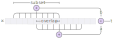
\includegraphics[scale=1]{graphics/function_task_static_problem.pdf}
\caption{Lorem Ipsum.}
\end{figure}

\subsubsection{Simple multiplication task}
\begin{table}[!h]

\caption{\label{tab:very-simple-function-results}Comparison of the success-rate, when the model converged, and the sparsity error for all weight matrices, with 95\% confidence interval on the $t = (x_1 + x_2) \cdot (x_1 + x_2 + x_3 + x_4)$ task. Each value is a summary of 100 different seeds.}
\centering
\begin{tabular}{crllll}
\toprule
\multicolumn{1}{c}{Op} & \multicolumn{1}{c}{Model} & \multicolumn{1}{c}{Success} & \multicolumn{2}{c}{Solved at} & \multicolumn{1}{c}{Sparsity error} \\
\cmidrule(l{3pt}r{3pt}){1-1} \cmidrule(l{3pt}r{3pt}){2-2} \cmidrule(l{3pt}r{3pt}){3-3} \cmidrule(l{3pt}r{3pt}){4-5} \cmidrule(l{3pt}r{3pt}){6-6}
 &  & Rate & Median & Mean & Mean\\
\midrule
 & $\mathrm{NAC}_{\bullet}$ & $13\% {~}^{+8\%}_{-5\%}$ & $5.5 \cdot 10^{4}$ & $5.9 \cdot 10^{4} {~}^{+7.8 \cdot 10^{3}}_{-6.6 \cdot 10^{3}}$ & $7.5 \cdot 10^{-6} {~}^{+2.0 \cdot 10^{-6}}_{-2.0 \cdot 10^{-6}}$\\

\nopagebreak
 & NALU & $26\% {~}^{+9\%}_{-8\%}$ & $7.0 \cdot 10^{4}$ & $7.8 \cdot 10^{4} {~}^{+6.2 \cdot 10^{3}}_{-8.6 \cdot 10^{3}}$ & $9.2 \cdot 10^{-6} {~}^{+1.7 \cdot 10^{-6}}_{-1.7 \cdot 10^{-6}}$\\

\nopagebreak
\multirow{-3}{*}{\centering\arraybackslash $\bm{\times}$} & NMU & $\mathbf{94\%} {~}^{+3\%}_{-6\%}$ & $\mathbf{1.4 \cdot 10^{4}}$ & $\mathbf{1.4 \cdot 10^{4}} {~}^{+2.2 \cdot 10^{2}}_{-2.1 \cdot 10^{2}}$ & $\mathbf{2.6 \cdot 10^{-8}} {~}^{+6.4 \cdot 10^{-9}}_{-6.4 \cdot 10^{-9}}$\\
\bottomrule
\end{tabular}
\end{table}


\subsubsection{Static function task - defaults}
% latex table generated in R 3.4.3 by xtable 1.8-3 package
% Fri May 10 17:19:56 2019
\begin{table}[H]
\centering
\caption{Shows the sucess-rate for extrapolation < $\epsilon$, at what global step the model converged at, and the sparse error for all weight matrices.} 
\begin{tabular}{lll |rrr}
  \hline
                      &                            & & \multicolumn{1}{l}{          converged.at} & \multicolumn{1}{l}{          sparse.error} & \multicolumn{1}{l}{          success.rate} \\ 
  operation            & model                      &     & \multicolumn{1}{l}{                      } & \multicolumn{1}{l}{                      } & \multicolumn{1}{l}{                      } \\ 
   \hline
  ${a \cdot b}$        & ${\mathrm{NAC}_\bullet}$ &     & $3371250$             & $8.0 \times 10^{-5}$ & $40\%$               \\ 
                       & NALU                       &     & ---                   &      ---              & $0\%$                   \\ 
                       & NMU                        &     & $1571900$             & $1.6 \times 10^{-4}$ & $100\%$              \\ \hline
  $a - b$              & ${\mathrm{NAC}_{+}}$      &     & $6300$                & $1.1 \times 10^{-1}$ & $100\%$              \\ 
                       & linear                     &     & $3300$                & $7.6 \times 10^{-2}$ & $100\%$              \\ 
                       & NALU                       &     & $1963250$             & $9.1 \times 10^{-2}$ & $40\%$               \\ 
                       & NAU                        &     & $3700$                & $4.3 \times 10^{-4}$ & $100\%$              \\ \hline 
  $a + b$              & ${\mathrm{NAC}_{+}}$      &     & $42900$               & $1.4 \times 10^{-1}$ & $100\%$              \\ 
                       & linear                     &     & $21300$               & $1.9 \times 10^{-1}$ & $100\%$              \\ 
                       & NALU                       &     & $81000$               & $1.9 \times 10^{-1}$ & $10\%$               \\ 
                       & NAU                        &     & $15500$               & $1.1 \times 10^{-4}$ & $100\%$              \\ 
   \hline
\end{tabular}
\end{table}


\subsubsection{Static function task - boundary}
\begin{figure}[H]
\centering
\includegraphics[width=\linewidth]{results/simple_function_static_input_size.pdf}
\caption{Lorem Ipsum.}
\end{figure}

\begin{figure}[H]
\centering
\includegraphics[width=\linewidth]{results/simple_function_static_overlap.pdf}
\caption{Lorem Ipsum.}
\end{figure}

\begin{figure}[H]
\centering
\includegraphics[width=\linewidth]{results/simple_function_static_subset.pdf}
\caption{Lorem Ipsum.}
\end{figure}

\subsection{sequential MNIST}

\begin{figure}[H]
\centering
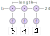
\includegraphics[scale=1]{graphics/mnist_sequence_problem.pdf}
\caption{Lorem Ipsum.}
\end{figure}


\section{Related work}

Lorem ipsum dolor sit amet, consectetur adipiscing elit. Ut mollis consequat lacus ac aliquam. Phasellus pharetra laoreet mi ac dignissim. Sed condimentum venenatis mollis. Nunc tempus arcu fermentum, viverra nisi non, bibendum tortor. Vestibulum in elit velit. In faucibus egestas est, in blandit dui interdum ut. Quisque felis odio, aliquet id congue non, hendrerit id dui. Fusce mattis diam condimentum augue aliquam, eu bibendum ex tempus. Vestibulum suscipit metus sed tortor scelerisque interdum. Nam laoreet purus dolor, in ornare augue dignissim eu. In hac habitasse platea dictumst. Lorem ipsum dolor sit amet, consectetur adipiscing elit. In ut diam nec nisi rhoncus finibus. Maecenas vel ligula vel metus ullamcorper auctor. Pellentesque volutpat quam sed ligula consectetur, ac facilisis purus facilisis.

Phasellus bibendum imperdiet mattis. Cras dictum purus nulla, sed finibus dolor porttitor sed. Proin in velit leo. Curabitur maximus, diam vel consectetur consequat, velit dolor vestibulum mi, eu consectetur felis mauris in justo. Donec non iaculis velit, quis egestas ex. Nullam consequat eros at nisi varius ultrices. Duis ultricies risus ac dolor semper tempor.

%Sed faucibus blandit enim, id faucibus dolor varius a. Pellentesque habitant morbi tristique senectus et netus et malesuada fames ac turpis egestas. Mauris ac aliquam justo, non hendrerit nunc. Fusce porttitor sodales efficitur. Vivamus egestas turpis sed posuere consequat. Nullam ut lectus ac nibh lacinia venenatis eu ut ipsum. Sed vitae egestas magna, a porta sem. Vivamus ac nulla quam. Pellentesque luctus sapien at erat vulputate, eu malesuada urna lobortis. Nam commodo molestie purus nec venenatis. Aliquam efficitur consequat dolor ut luctus. Interdum et malesuada fames ac ante ipsum primis in faucibus. Aenean at congue metus. Vivamus dolor sapien, suscipit a urna quis, sodales aliquam ligula. Donec elementum, est in mollis dictum, nunc risus iaculis mi, at tempus ex enim id risus.


% NALU gating issues, use a "model selection" theory (Alexander stuff).

% 1. Differentiable Subset Sampling  https://arxiv.org/abs/1901.10517v1
% 

\section{Conclusion}

% Far better sucess-rate, learns faster, have discrete weights.
% NAC-mul, converges only 13% of the time on a very simple problem. Our NMU converges 94% of the time.
% We tested on a range of different dataset configurations and shown that this is generally the case.

% NMU, understands negative inputs and thus can extrapolate into that domain.
% NAU, produces discrete weights unlike NAC.

% The models are theoretically inspired.

% MNIST findings?

\subsubsection*{Acknowledgments}

\xblackout{We would like to thank Andrew Trask and the other authors of the NALU paper, for highlighting the importance and challenges of etrapolation in Neural Networks. We would also like to thank the students Raja Shan Zaker Kreen and William Frisch Moller from The Technical University of Denmark, who showed us that the NALU does not converge consistently.}

\bibliographystyle{plainnat}
\bibliography{bibliography}

\newpage
\appendix
\section{Gradient derivatives}

\subsection{Weight matrix construction}

The gradient of the weight matrix construction $\mathrm{tahn}({\hat{\mathbf{W}}}) \sigma({\hat{\mathbf{M}}})$ is straight forward to derive.



\begin{equation}
\begin{aligned}
\frac{\partial\mathcal{L}}{\partial \hat{W}_{h_\ell, h_{\ell-1}}} &= \frac{\partial\mathcal{L}}{\partial W_{h_\ell, h_{\ell-1}}} \frac{\partial W_{h_\ell, h_{\ell-1}}}{\partial \hat{W}_{h_\ell, h_{\ell-1}}} \\
&= \frac{\partial\mathcal{L}}{\partial W_{h_\ell, h_{\ell-1}}} (1 - \tanh^2(\hat{W}_{h_\ell, h_{\ell-1}})) \sigma(\hat{M}_{h_\ell, h_{\ell-1}}) \\
\frac{\partial\mathcal{L}}{\partial \hat{M}_{h_\ell, h_{\ell-1}}} &= \frac{\partial\mathcal{L}}{\partial W_{h_\ell, h_{\ell-1}}} \frac{\partial W_{h_\ell, h_{\ell-1}}}{\partial \hat{M}_{h_\ell, h_{\ell-1}}} \\
&= \frac{\partial\mathcal{L}}{\partial W_{h_\ell, h_{\ell-1}}} \tanh(\hat{W}_{h_\ell, h_{\ell-1}}) \sigma(\hat{M}_{h_\ell, h_{\ell-1}}) (1 - \sigma(\hat{M}_{h_\ell, h_{\ell-1}}))
\end{aligned}
\end{equation}

\subsection{Multiplication gradient}

\begin{equation}
\begin{aligned}
\frac{\partial z_{h_\ell}}{\partial W_{h_\ell, h_{\ell-1}}} &= \exp\left(\sum_{h'_{\ell-1}=1}^{H_{\ell-1}} W_{h_{\ell}, h'_{\ell-1}} \log(|z_{h'_{\ell-1}}| + \epsilon) \right) \log(|z_{h_{\ell-1}}| + \epsilon)
\end{aligned}
\end{equation}
\section{Moments}

\subsection{Expectation and variance for weight matrix construction in NAC layers}

The weight matrix construction in NAC, is defined in scalar notation as: 
\begin{equation}
W_{h_\ell, h_{\ell-1}} = \tanh(\hat{W}_{h_\ell, h_{\ell-1}}) \sigma(\hat{M}_{h_\ell, h_{\ell-1}})
\end{equation}

Simplifying the notation of this, and re-expressing it using stochastic variables with uniform distributions this can be written as:
\begin{equation}
\begin{aligned}
W &\sim \tanh(\hat{W}) \sigma(\hat{M}) \\
\hat{W} &\sim ~ U[-r, r] \\
\hat{M} &\sim ~ U[-r, r] 
\end{aligned}
\end{equation}

Since $\tanh({\hat{W}})$ is an odd-function and $E[\hat{W}] = 0$, deriving the expectation $E[W]$ is trivial.
\begin{equation}
\mathrm{E}[W] = \mathrm{E}[\tanh(\hat{W})]\mathrm{E}[\sigma(\hat{M})] = 0 \cdot \mathrm{E}[\sigma(\hat{M})] = 0
\end{equation}

The variance is more complicated, however as $\hat{W}$ and $\hat{M}$ are independent, it can be simplified to:
\begin{equation}
\mathrm{Var}[W] = \mathrm{E}[\tanh(\hat{W})^2] \mathrm{E}[\sigma(\hat{M})^2] - \mathrm{E}[\tanh(\hat{W})]^2 \mathrm{E}[\sigma(\hat{M})]^2 = \mathrm{E}[\tanh(\hat{W})^2] \mathrm{E}[\sigma(\hat{M})^2]
\end{equation}

These second moments can be analyzed independently. First for $\mathrm{E}[\tanh(\hat{W})^2]$:
\begin{equation}
\begin{aligned}
\mathrm{E}[\tanh(\hat{W})^2] &= \int_{-\infty}^{\infty} \tanh(x)^2 f_{U[-r, r]}(x)\ \mathrm{d}x \\
&= \frac{1}{2r} \int_{-r}^{r} \tanh(x)^2\ \mathrm{d}x \\
&= \frac{1}{2r} \cdot 2 \cdot (r - \tanh(r)) \\
&= 1 - \frac{\tanh(r)}{r}
\end{aligned}
\end{equation}

Then for $\mathrm{E}[\tanh(\hat{M})^2]$:
\begin{equation}
\begin{aligned}
\mathrm{E}[\sigma(\hat{M})^2] &= \int_{-\infty}^{\infty} \sigma(x)^2 f_{U[-r, r]}(x)\ \mathrm{d}x \\
&= \frac{1}{2r} \int_{-r}^{r} \sigma(x)^2\ \mathrm{d}x \\
&= \frac{1}{2r} \left(r - \tanh\left(\frac{r}{2}\right)\right)
\end{aligned}
\end{equation}

Finally this gives the variance:
\begin{equation}
\mathrm{Var}[W] = \frac{1}{2r} \left(1 - \frac{\tanh(r)}{r}\right) \left(r - \tanh\left(\frac{r}{2}\right)\right)
\end{equation}

\subsection{Expectation and variance of $\mathrm{NAC}_{\bullet}$}
\subsubsection{Forward pass}
Assuming that each $z_{h_{\ell-1}}$ are independent the expectation can be simplified to:
\begin{equation}
\begin{aligned}
E[z_{h_\ell}] &= E\left[\exp\left(\sum_{h_{\ell-1}=1}^{H_{\ell-1}} W_{h_{\ell}, h_{\ell-1}} \log(|z_{h_{\ell-1}}| + \epsilon) \right)\right] \\
&= E\left[\prod_{h_{\ell-1}=1}^{H_{\ell-1}} \exp(W_{h_{\ell}, h_{\ell-1}} \log(|z_{h_{\ell-1}}| + \epsilon)) \right] \\
&= \prod_{h_{\ell-1}=1}^{H_{\ell-1}} E[\exp(W_{h_{\ell}, h_{\ell-1}} \log(|z_{h_{\ell-1}}| + \epsilon))] \\
&= E[\exp(W_{h_{\ell}, h_{\ell-1}} \log(|z_{h_{\ell-1}}| + \epsilon))]^{H_{\ell-1}} \\
&= E\left[(|z_{h_{\ell-1}}| + \epsilon)^{W_{h_{\ell}, h_{\ell-1}}}\right]^{H_{\ell-1}} \\
&= E\left[f(z_{h_{\ell-1}}, W_{h_{\ell}, h_{\ell-1}})\right]^{H_{\ell-1}}
\end{aligned}
\end{equation}

Here we define $f$ as a non-linear transformation function of two independent stocastic variables:
\begin{equation}
f(z_{h_{\ell-1}}, W_{h_{\ell}, h_{\ell-1}}) = (|z_{h_{\ell-1}}| + \epsilon)^{W_{h_{\ell}, h_{\ell-1}}}
\end{equation}

We then take the second order taylor approximation of $f$, around $(E[z_{h_{\ell-1}}], E[W_{h_{\ell}, h_{\ell-1}}])$.
\begin{equation}
\begin{aligned}
&E[f(z_{h_{\ell-1}}, W_{h_{\ell}, h_{\ell-1}})] \approx
E\Bigg[\\
&f(E[z_{h_{\ell-1}}], E[W_{h_{\ell}, h_{\ell-1}}])\\
&+ \begin{bmatrix}
z_{h_{\ell-1}} - E[z_{h_{\ell-1}}] \\ W_{h_{\ell}, h_{\ell-1}} - E[W_{h_{\ell}, h_{\ell-1}}]
\end{bmatrix}^T \begin{bmatrix}
\frac{\partial f(z_{h_{\ell-1}}, W_{h_{\ell}, h_{\ell-1}})}{\partial z_{h_{\ell-1}}} \\
\frac{\partial f(z_{h_{\ell-1}}, W_{h_{\ell}, h_{\ell-1}})}{\partial W_{h_{\ell}, h_{\ell-1}}}
\end{bmatrix} \Bigg\rvert_{
\begin{cases}
z_{h_{\ell-1}} = E[z_{h_{\ell-1}}] \\
W_{h_{\ell}, h_{\ell-1}} = E[W_{h_{\ell}, h_{\ell-1}}]
\end{cases}
} \\
&+ \frac{1}{2} \begin{bmatrix}
z_{h_{\ell-1}} - E[z_{h_{\ell-1}}] \\ W_{h_{\ell}, h_{\ell-1}} - E[W_{h_{\ell}, h_{\ell-1}}]
\end{bmatrix}^T \\
&\bullet \begin{bmatrix}
\frac{\partial^2 f(z_{h_{\ell-1}}, W_{h_{\ell}, h_{\ell-1}})}{\partial^2 z_{h_{\ell-1}}} & \frac{\partial^2 f(z_{h_{\ell-1}}, W_{h_{\ell}, h_{\ell-1}})}{\partial z_{h_{\ell-1}} \partial W_{h_{\ell}, h_{\ell-1}}} \\
\frac{\partial^2 f(z_{h_{\ell-1}}, W_{h_{\ell}, h_{\ell-1}})}{\partial z_{h_{\ell-1}} \partial W_{h_{\ell}, h_{\ell-1}}} & \frac{\partial^2 f(z_{h_{\ell-1}}, W_{h_{\ell}, h_{\ell-1}})}{\partial^2 W_{h_{\ell}, h_{\ell-1}}}
\end{bmatrix} \Bigg\rvert_{
\begin{cases}
z_{h_{\ell-1}} = E[z_{h_{\ell-1}}] \\
W_{h_{\ell}, h_{\ell-1}} = E[W_{h_{\ell}, h_{\ell-1}}]
\end{cases}
} \\
&\bullet \begin{bmatrix}
z_{h_{\ell-1}} - E[z_{h_{\ell-1}}] \\ W_{h_{\ell}, h_{\ell-1}} - E[W_{h_{\ell}, h_{\ell-1}}]
\end{bmatrix}\Bigg]
\end{aligned}
\end{equation}

Because $E[z_{h_{\ell-1}} - E[z_{h_{\ell-1}}]] = 0$, $E[W_{h_{\ell}, h_{\ell-1}} - E[W_{h_{\ell}, h_{\ell-1}}]] = 0$, and $Cov[z_{h_{\ell-1}}, W_{h_{\ell}, h_{\ell-1}}] = 0$. This similifies to:
\begin{equation}
\begin{aligned}
&E[f(z_{h_{\ell-1}}, W_{h_{\ell}, h_{\ell-1}})] \approx
f(E[z_{h_{\ell-1}}], E[W_{h_{\ell}, h_{\ell-1}}])\\
&+ \frac{1}{2} Var\begin{bmatrix}
z_{h_{\ell-1}} \\ W_{h_{\ell}, h_{\ell-1}}
\end{bmatrix}^T \begin{bmatrix}
\frac{\partial^2 f(z_{h_{\ell-1}}, W_{h_{\ell}, h_{\ell-1}})}{\partial^2 z_{h_{\ell-1}}} \\
\frac{\partial^2 f(z_{h_{\ell-1}}, W_{h_{\ell}, h_{\ell-1}})}{\partial^2 W_{h_{\ell}, h_{\ell-1}}}
\end{bmatrix} \Bigg\rvert_{
\begin{cases}
z_{h_{\ell-1}} = E[z_{h_{\ell-1}}] \\
W_{h_{\ell}, h_{\ell-1}} = E[W_{h_{\ell}, h_{\ell-1}}]
\end{cases}
}
\end{aligned}
\end{equation}

Inserting the derivatives and computing the inner products yields:
\begin{equation}
\begin{aligned}
&E[f(z_{h_{\ell-1}}, W_{h_{\ell}, h_{\ell-1}})] \approx
(|E[z_{h_{\ell-1}}]| + \epsilon)^{E[W_{h_{\ell}, h_{\ell-1}}]} \\
&+ \frac{1}{2} Var[z_{h_{\ell-1}}] (|E[z_{h_{\ell-1}}]| + \epsilon)^{E[W_{h_{\ell}, h_{\ell-1}}] - 2} E[W_{h_{\ell}, h_{\ell-1}}] (E[W_{h_{\ell}, h_{\ell-1}}] - 1) \\
&+ \frac{1}{2} Var[W_{h_{\ell}, h_{\ell-1}}] (|E[z_{h_{\ell-1}}]| + \epsilon)^{E[W_{h_{\ell}, h_{\ell-1}}]} \log(|E[z_{h_{\ell-1}}]| + \epsilon)^2 \\
&=1 + \frac{1}{2} Var[W_{h_{\ell}, h_{\ell-1}}] \log(|E[z_{h_{\ell-1}}]| + \epsilon)^2
\end{aligned}
\end{equation}

This gives the final expectation:
\begin{equation}
\begin{aligned}
E[z_{h_\ell}] &= E\left[f(z_{h_{\ell-1}}, W_{h_{\ell}, h_{\ell-1}})\right]^{H_{\ell-1}} \\
&\approx\left(1 + \frac{1}{2} Var[W_{h_{\ell}, h_{\ell-1}}] \log(|E[z_{h_{\ell-1}}]| + \epsilon)^2\right)^{H_{\ell-1}}
\end{aligned}
\end{equation}

As this expectation is of particular interrest, we evaluate the error of the approximation, where $W_{h_{\ell}, h_{\ell-1}} \sim U[-r_w,r_w]$ and $z_{h_{\ell-1}} \sim U[0, r_z]$. These distributions are what is used in the simple function task is done.  The result is seen in figure \ref{fig:nac-mul-expectation-estimate}.
\begin{figure}[h]
\centering
\includegraphics[width=\linewidth]{graphics/nac-mul-expectation-estimate.pdf}
\caption{Error between theoretical approximation and the numerical approximation estimated by random sampling of $100000$ observations at each combination of $r_z$ and $r_w$.}
\label{fig:nac-mul-expectation-estimate}
\end{figure}

The variance can be derived using the same assumptions about expectation and no correlation.
\begin{equation}
\begin{aligned}
Var[z_{h_\ell}] &= E[z_{h_\ell}^2] - E[z_{h_\ell}]^2 \\
&= E\left[\prod_{h_{\ell-1}=1}^{H_{\ell-1}} (|z_{h_{\ell-1}}| + \epsilon)^{2 \cdot W_{h_{\ell}, h_{\ell-1}}} \right]
- E\left[\prod_{h_{\ell-1}=1}^{H_{\ell-1}} (|z_{h_{\ell-1}}| + \epsilon)^{W_{h_{\ell}, h_{\ell-1}}}\right]^2 \\
&= E\left[f(z_{h_{\ell-1}}, 2 \cdot W_{h_{\ell}, h_{\ell-1}}) \right]^{H_{\ell-1}}
- E\left[f(z_{h_{\ell-1}}, W_{h_{\ell}, h_{\ell-1}})\right]^{2\cdot H_{\ell-1}}
\end{aligned}
\end{equation}

We already have from the expectation result that:
\begin{equation}
E\left[f(z_{h_{\ell-1}}, W_{h_{\ell}, h_{\ell-1}})\right] \approx 1 + \frac{1}{2} Var[W_{h_{\ell}, h_{\ell-1}}] \log(|E[z_{h_{\ell-1}}]| + \epsilon)^2
\end{equation}

By substitution of variable we have that:
\begin{equation}
\begin{aligned}
E\left[f(z_{h_{\ell-1}}, 2 \cdot W_{h_{\ell}, h_{\ell-1}})\right] &\approx 1 + \frac{1}{2} Var[2 \cdot W_{h_{\ell}, h_{\ell-1}}] \log(|E[z_{h_{\ell-1}}]| + \epsilon)^2 \\
&= \approx 1 + 2 \cdot Var[W_{h_{\ell}, h_{\ell-1}}] \log(|E[z_{h_{\ell-1}}]| + \epsilon)^2
\end{aligned}
\end{equation}

This gives the variance:
\begin{equation}
\begin{aligned}
Var[z_{h_\ell}] &= E\left[f(z_{h_{\ell-1}}, 2 \cdot W_{h_{\ell}, h_{\ell-1}}) \right]^{H_{\ell-1}}
- E\left[f(z_{h_{\ell-1}}, W_{h_{\ell}, h_{\ell-1}})\right]^{2\cdot H_{\ell-1}} \\
&\approx \left(1 + 2 \cdot Var[W_{h_{\ell}, h_{\ell-1}}] \log(|E[z_{h_{\ell-1}}]| + \epsilon)^2\right)^{H_{\ell-1}} \\
&- \left(1 + \frac{1}{2} \cdot Var[W_{h_{\ell}, h_{\ell-1}}] \log(|E[z_{h_{\ell-1}}]| + \epsilon)^2\right)^{2\cdot H_{\ell-1}}
\end{aligned}
\end{equation}

\subsubsection{Backward pass}

The expectation of the backpropagation term:
\begin{equation}
E[\delta_{h_\ell}] = E\left[\sum_{h_{\ell+1}=1}^{H_{\ell+1}} \delta_{h_{\ell+1}} \frac{\partial z_{h_{\ell+1}}}{\partial z_{h_\ell}}\right] = H_{\ell+1} E[\delta_{h_{\ell+1}}] E\left[\frac{\partial z_{h_{\ell+1}}}{\partial z_{h_\ell}}\right]
\end{equation}

Where we have that:
\begin{equation}
E\left[\frac{\partial z_{h_{\ell+1}}}{\partial z_{h_\ell}}\right] = E[{h_{\ell+1}}] E[W_{h_{\ell+1}, h_{\ell}}] E\left[ \frac{\mathrm{abs}'(z_{h_{\ell}})}{|z| + \epsilon}\right] = E[m_{h_{\ell+1}}] \cdot 0 \cdot E\left[ \frac{\mathrm{abs}'(z_{h_{\ell}})}{|z| + \epsilon}\right] = 0
\end{equation}

Deriving the variance is more complicated as:
\begin{equation}
\begin{aligned}
Var\left[\frac{\partial m_{h_{\ell+1}}}{\partial z_{h_\ell}}\right] &= Var\left[m_{h_{\ell+1}} W_{h_{\ell+1}, h_{\ell}} \frac{\mathrm{abs}'(z_{h_{\ell}})}{|z_{h_{\ell}}| + \epsilon}\right]
\end{aligned}
\end{equation}

Assuming independence between each term this can be simplified to as:
\begin{equation}
\begin{aligned}
Var\left[\frac{\partial z_{h_{\ell+1}}}{\partial z_{h_\ell}}\right] &= E[z_{h_{\ell+1}}^2] E[W_{h_{\ell+1}, h_{\ell}}^2] E\left[\left( \frac{\mathrm{abs}'(z_{h_{\ell}})}{|z_{h_{\ell}}| + \epsilon}\right)^2\right] \\
&- E[z_{h_{\ell+1}}]^2 E[W_{h_{\ell+1}, h_{\ell}}]^2 E\left[ \frac{\mathrm{abs}'(z_{h_{\ell}})}{|z_{h_{\ell}}| + \epsilon}\right]^2 \\
&= E[z_{h_{\ell+1}}^2] Var[W_{h_{\ell+1}, h_{\ell}}] E\left[\left( \frac{\mathrm{abs}'(z_{h_{\ell}})}{|z_{h_{\ell}}| + \epsilon}\right)^2\right] \\
&- E[z_{h_{\ell+1}}]^2 \cdot 0 \cdot E\left[ \frac{\mathrm{abs}'(z_{h_{\ell}})}{|z_{h_{\ell}}| + \epsilon}\right]^2 \\
&= E[z_{h_{\ell+1}}^2] Var[W_{h_{\ell+1}, h_{\ell}}] E\left[\left( \frac{\mathrm{abs}'(z_{h_{\ell}})}{|z_{h_{\ell}}| + \epsilon}\right)^2\right]
\end{aligned}
\end{equation}

Using Taylor approximation around $E[z_{h_{\ell}}]$ we have:
\begin{equation}
\begin{aligned}
E\left[\left(\frac{\mathrm{abs}'(z_{h_{\ell}})}{|z| + \epsilon}\right)^2\right] &\approx\frac{1}{\left(|E[z_{h_{\ell}}]| + \epsilon\right)^2} + \frac{1}{2} \frac{6}{\left(|E[z_{h_{\ell}}]| + \epsilon\right)^4} Var[z_{h_{\ell}}] \\
&= \frac{1}{\left(|E[z_{h_{\ell}}]| + \epsilon\right)^2} + \frac{3}{\left(|E[z_{h_{\ell}}]| + \epsilon\right)^4} Var[z_{h_{\ell}}]
\end{aligned}
\end{equation}

Also reusing the result for $E[z_{h_\ell}^2]$ from earlier the variance can be expressed as:
\begin{equation}
\begin{aligned}
Var\left[\frac{\partial \mathcal{L}}{\partial z_{h_{\ell-1}}}\right] &\approx Var\left[\frac{\partial \mathcal{L}}{\partial z_{h_{\ell}}}\right] H_{\ell}\ \left(1 + 2 \cdot Var[W_{h_{\ell}, h_{\ell-1}}] \log(|E[z_{h_{\ell-1}}]| + \epsilon)^2\right)^{H_{\ell-1}} \\
&\cdot Var[W_{h_{\ell}, h_{\ell-1}}] \left(\frac{1}{\left(|E[z_{h_{\ell-1}}]| + \epsilon\right)^2} + \frac{3}{\left(|E[z_{h_{\ell-1}}]| + \epsilon\right)^4} Var[z_{h_{\ell-1}}]\right)
\end{aligned}
\end{equation}

\subsection{Expectation and variance of NMU}

\subsubsection{Forward pass}

Assuming that each $z_{h_{\ell-1}}$ are independent, that $E[z_{h_{\ell-1}}] = 0$, and that $E[W_{h_{\ell-1},h_\ell}] = \nicefrac{1}{2}$ the expectation is:
\begin{equation}
\begin{aligned}
E[z_{h_\ell}] &\approx E\left[\prod_{h_{\ell-1}=1}^{H_{\ell-1}} \left(W_{h_{\ell-1},h_\ell} z_{h_{\ell-1}} + 1 - W_{h_{\ell-1},h_\ell} \right)\right] \\
&\approx E\left[W_{h_{\ell-1},h_\ell} z_{h_{\ell-1}} + 1 - W_{h_{\ell-1},h_\ell} \right]^{H_{\ell-1}} \\
&\approx \left(E[W_{h_{\ell-1},h_\ell}] E[z_{h_{\ell-1}}] + 1 - E[W_{h_{\ell-1},h_\ell}] \right)^{H_{\ell-1}} \\
&\approx\left(\frac{1}{2}\cdot0 + 1 - \frac{1}{2}\right)^{H_{\ell-1}} \\
&\approx\left(\frac{1}{2}\right)^{H_{\ell-1}}
\end{aligned}
\end{equation}

Using the same assumptions for the variance one gets:
\begin{equation}
\begin{aligned}
Var[z_{h_\ell}] &= E[z_{h_\ell}^2] - E[z_{h_\ell}]^2 \\
&\approx E[z_{h_\ell}^2] - \left(\frac{1}{2}\right)^{2 \cdot H_{\ell-1}} \\
&\approx E\left[\prod_{h_{\ell-1}=1}^{H_{\ell-1}}\left(W_{h_{\ell-1},h_\ell} z_{h_{\ell-1}} + 1 - W_{h_{\ell-1},h_\ell}\right)^2\right] - \left(\frac{1}{2}\right)^{2 \cdot H_{\ell-1}} \\
&\approx E[\left(W_{h_{\ell-1},h_\ell} z_{h_{\ell-1}} + 1 - W_{h_{\ell-1},h_\ell}\right)^2]^{H_{\ell-1}}- \left(\frac{1}{2}\right)^{2 \cdot H_{\ell-1}} \\
&\approx \Big(E[W_{h_{\ell-1},h_\ell}^2] E[z_{h_{\ell-1}}^2] - 2 E[W_{h_{\ell-1},h_\ell}^2] E[z_{h_{\ell-1}}] \\
&\quad\quad+ E[W_{h_{\ell-1},h_\ell}^2] + 2 E[W_{h_{\ell-1},h_\ell}] E[z_{h_{\ell-1}}] \\
&\quad\quad- 2 E[W_{h_{\ell-1},h_\ell}] + 1\Big)^{H_{\ell-1}}- \left(\frac{1}{2}\right)^{2 \cdot H_{\ell-1}} \\
&\approx \Big(E[W_{h_{\ell-1},h_\ell}^2] E[z_{h_{\ell-1}}^2] + E[W_{h_{\ell-1},h_\ell}^2] \\
&\quad\quad- 2 E[W_{h_{\ell-1},h_\ell}] + 1\Big)^{H_{\ell-1}}- \left(\frac{1}{2}\right)^{2 \cdot H_{\ell-1}} \\
&= \left(E[W_{h_{\ell-1},h_\ell}^2] \left(E[z_{h_{\ell-1}}^2] + 1\right)\right)^{H_{\ell-1}}- \left(\frac{1}{2}\right)^{2 \cdot H_{\ell-1}} \\
&\approx \left(\left(Var[W_{h_{\ell-1},h_\ell}] + E[W_{h_{\ell-1},h_\ell}]^2\right) \left(Var[z_{h_{\ell-1}}] + 1\right)\right)^{H_{\ell-1}}- \left(\frac{1}{2}\right)^{2 \cdot H_{\ell-1}} \\
&= \left(Var[W_{h_{\ell-1},h_\ell}] + \frac{1}{4}\right)^{H_{\ell-1}} \left(Var[z_{h_{\ell-1}}] + 1\right)^{H_{\ell-1}} - \left(\frac{1}{2}\right)^{2 \cdot H_{\ell-1}}
\end{aligned}
\end{equation}

\subsubsection{Backward pass}

For the backward pass the expectation can using the same assumptions be derived to:
\begin{equation}
\begin{aligned}
E\left[\frac{\partial \mathcal{L}}{\partial z_{h_{\ell-1}}}\right]
&= H_\ell E\left[\frac{\partial \mathcal{L}}{\partial z_{h_\ell}} \frac{\partial z_{h_\ell}}{\partial z_{h_{\ell-1}}}\right] \\
&= H_\ell E\left[\frac{\partial \mathcal{L}}{\partial z_{h_\ell}}\right] E\left[\frac{\partial z_{h_\ell}}{\partial z_{h_{\ell-1}}}\right] \\
&= H_\ell E\left[\frac{\partial \mathcal{L}}{\partial z_{h_\ell}}\right] E\left[\frac{z_{h_\ell}}{W_{h_{\ell-1},h_\ell} z_{h_{\ell-1}} + 1 - W_{h_{\ell-1},h_\ell}} W_{h_{\ell-1},h_\ell}\right] \\
&= H_\ell E\left[\frac{\partial \mathcal{L}}{\partial z_{h_\ell}}\right] E\left[\frac{z_{h_\ell}}{W_{h_{\ell-1},h_\ell} z_{h_{\ell-1}} + 1 - W_{h_{\ell-1},h_\ell}}\right]E\left[W_{h_{\ell-1},h_\ell}\right] \\
&= H_\ell E\left[\frac{\partial \mathcal{L}}{\partial z_{h_\ell}}\right] \left(\frac{1}{2}\right)^{H_{\ell-1}-1} \frac{1}{2} \\
&= E\left[\frac{\partial \mathcal{L}}{\partial z_{h_\ell}}\right] H_\ell \left(\frac{1}{2}\right)^{H_{\ell-1}} \\
&\approx 0 \cdot H_\ell \cdot \left(\frac{1}{2}\right)^{H_{\ell-1}} \\
&= 0
\end{aligned}
\end{equation}


And finally the variance for the backward pass is derived using the same assumptions.
\begin{equation}
\begin{aligned}
Var&\left[\frac{\partial \mathcal{L}}{\partial z_{h_{\ell-1}}}\right] = H_\ell Var\left[\frac{\partial \mathcal{L}}{\partial z_{h_\ell}} \frac{\partial z_{h_\ell}}{\partial z_{h_{\ell-1}}}\right] \\
&= H_\ell \Bigg(Var\left[\frac{\partial \mathcal{L}}{\partial z_{h_\ell}}\right] E\left[\frac{\partial z_{h_\ell}}{\partial z_{h_{\ell-1}}}\right]^2 + E\left[\frac{\partial \mathcal{L}}{\partial z_{h_\ell}}\right]^2 Var\left[\frac{\partial z_{h_\ell}}{\partial z_{h_{\ell-1}}}\right] \\
&+ Var\left[\frac{\partial \mathcal{L}}{\partial z_{h_\ell}}\right] Var\left[\frac{\partial z_{h_\ell}}{\partial z_{h_{\ell-1}}}\right]\Bigg) \\
&\approx Var\left[\frac{\partial \mathcal{L}}{\partial z_{h_\ell}}\right] H_\ell Var\left[\frac{\partial z_{h_\ell}}{\partial z_{h_{\ell-1}}}\right] \\
&\approx Var\left[\frac{\partial \mathcal{L}}{\partial z_{h_\ell}}\right] H_\ell \Bigg( E\left[\left(\frac{z_{h_\ell}}{W_{h_{\ell-1},h_\ell} z_{h_{\ell-1}} + 1 - W_{h_{\ell-1},h_\ell}}\right)^2\right] E[W_{h_{\ell-1},h_\ell}^2] \\
&- E\left[\frac{z_{h_\ell}}{W_{h_{\ell-1},h_\ell} z_{h_{\ell-1}} + 1 - W_{h_{\ell-1},h_\ell}}\right]^2 E[W_{h_{\ell-1},h_\ell}]^2 \Bigg) \\
&\approx Var\left[\frac{\partial \mathcal{L}}{\partial z_{h_\ell}}\right] H_\ell \Bigg( E\left[\left(\frac{z_{h_\ell}}{W_{h_{\ell-1},h_\ell} z_{h_{\ell-1}} + 1 - W_{h_{\ell-1},h_\ell}}\right)^2\right] E[W_{h_{\ell-1},h_\ell}^2] \\
&- \left(\frac{1}{2}\right)^{2 \cdot \left(H_{\ell-1}-1\right)} \left(\frac{1}{2}\right)^2\Bigg) \\
&\approx Var\left[\frac{\partial \mathcal{L}}{\partial z_{h_\ell}}\right] H_\ell \Bigg( \left(\left(Var[W_{h_{\ell-1},h_\ell}] + \frac{1}{4}\right) \left(Var[z_{h_{\ell-1}}] + 1\right)\right)^{H_{\ell-1}-1} \\
&\cdot \left(Var[W_{h_{\ell-1},h_\ell}] + \frac{1}{4}\right) - \left(\frac{1}{2}\right)^{2 \cdot H_{\ell-1}}\Bigg) \\
&= Var\left[\frac{\partial \mathcal{L}}{\partial z_{h_\ell}}\right] H_\ell \Bigg( \left(Var[W_{h_{\ell-1},h_\ell}] + \frac{1}{4}\right)^{H_{\ell-1}} \left(Var[z_{h_{\ell-1}}] + 1\right)^{H_{\ell-1}-1} \\
&- \left(\frac{1}{2}\right)^{2 \cdot H_{\ell-1}}\Bigg)
\end{aligned}
\end{equation}

\subsubsection{Initialization}

The expectation of $W_{h_{\ell-1},h_\ell}$ should be $E[W_{h_{\ell-1},h_\ell}] = \frac{1}{2}$. Using the variance approximations found, the variance should be according to the forward pass:

\begin{equation}
Var[W_{h_{\ell-1},h_\ell}] = \left((1 + Var[z_{h_\ell}])^{-H_{\ell-1}}Var[z_{h_\ell}] + (4 + 4Var[z_{h_\ell}])^{-H_{\ell-1}}\right)^{\frac{1}{H_{\ell-1}}} - \frac{1}{4}
\end{equation}

And according to the backward pass it should be:
\begin{equation}
Var[W_{h_{\ell-1},h_\ell}] = \left(H_\ell (1 + Var[z_{h_{\ell-1}}]) (4 + 4 Var[z_{h_{\ell-1}}])^{-H_{\ell-1}} + (1 + Var[z_{h_{\ell-1}}])^{1 - H_{\ell-1}}\right)^{\frac{1}{H}} - \frac{1}{4}
\end{equation}

These are both dependent on the input variance. If the input variance is know then optimal initialization is possible. However, as this is often not the case one can perhaps assume that $Var[z_{h_{\ell-1}}] = 1$. This is not an unreasonable assumption in many cases, as there may either be a normalization layer somewhere or the input is normalized. If unit variance is assumed, one gets from the forward pass:
\begin{equation}
Var[W_{h_{\ell-1},h_\ell}] = \left(2^{-H_{\ell-1}} + 8^{-H_{\ell-1}}\right)^{\frac{1}{H_{\ell-1}}} - \frac{1}{4} = \frac{1}{8} \left(\left(4^{H_{\ell-1}} + 1\right)^{H_{\ell-1}} - 2\right)
\end{equation}

And from the backward pass:
\begin{equation}
Var[W_{h_{\ell-1},h_\ell}] = \left(2 H_\ell  8^{-H_{\ell-1}} + 2^{1 - H_{\ell-1}}\right)^{\frac{1}{H}} - \frac{1}{4}
\end{equation}

The variance requirement for the backward pass is hard to satisfy, as this is dependent on two variables. However, the variance requirement from the forward pass quickly $Var[W_{h_{\ell-1},h_\ell}] = \frac{1}{4}$ may be a reasonable initialization.


\section{Simple function task}
\subsection{Dataset generation}
\label{sec:appendix:simple-function-task:data-generation}
All datasets in the simple function task experiments are generated using the following algorithm:

\begin{algorithm}[H]
  \caption{Dataset sampling algorithm}
  \begin{algorithmic}[1]
    \Function{Dataset}{${\Call{Op}{\cdot, \cdot}: \mathrm{Operation}}$, ${i: \mathrm{Input Size}}$, ${s: \mathrm{Subset Ratio}}$, ${o: \mathrm{Overlap Ratio}}$, ${\hspace{3cm}R: \mathrm{Range}}$}
      \Let{$\mathbf{x}$}{\Call{Uniform}{$R_{lower}, R_{upper}, i$}} \Comment{Sample $i$ elements uniformly}
      \Let{$k$}{\Call{Uniform}{$0, 1 - 2s - o$}} \Comment{Sample offset}
      \Let{$a$}{\Call{Sum}{$\mathbf{x}[ik:i(k+s)]$}} \Comment{Create sum $a$ from subset}
      \Let{$b$}{\Call{Sum}{$\mathbf{x}[i(k+s-o):i (k+2s-0)]$}} \Comment{Create sum $b$ from subset}
      \Let{$t$}{\Call{Op}{$a, b$}} \Comment{Perform operation on $a$ and $b$}
      \State \Return{$x, t$}
    \EndFunction
  \end{algorithmic}
\end{algorithm}


\end{document}